\chapter{Friedmann-Gleichung\label{chapter:thema}}
\lhead{Friedmann-Gleichung}
\begin{refsection}
\chapterauthor{Andri Hartmann und Tobias Schuler}
\printbibliography[heading=subbibliography]

\lhead{Einleitung zur Friedmann-Gleichung}
\rhead{}
\begin{quote}
	\textit{Wir dürfen das Weltall nicht einengen, um es den Grenzen unseres Vorstellungsvermögens anzupassen, wie der Mensch es bisher zu tun pflegte. Wir müssen vielmehr unser Wissen ausdehnen, sodass es das Bild des Weltalls zu fassen vermag.}\footnote{Sir Francis von Verulam Bacon (1561 - 1626)}
\end{quote}
Das Universum ist ein sehr komplexes Gebilde. Wir versuchten, so gut es ging, uns mit der ganzen Materie auseinanderzusetzen. Dabei mussten wir feststellen, das "`Unwissen"' manchmal die bessere Variante als "`Verstehen"' ist. Versucht man die Friedmann-Gleichung mit all ihren Facetten zu verstehen, stösst man schnell auf Begriffe wie Tensoren, Allgemeine Relativitätstheorie, dunkle Energie usw. Diese Begriffe stellen Hürden dar, die mit unserem Wissen nur selten zu überwinden sind. Aufgeben war aber nie eine Option. "`Wir müssen unser Vorstellungsvermögen ausdehnen und nicht das Universum unserer Vorstellung anpassen"', wie Sir Francis sagt. Mit dieser Einstellung konnten wir sehr viel Neues über das Universum lernen. Wir hoffen, dass wir euch im folgenden Kapitel unsere neugewonnenen Erkenntnisse zeigen  und euch die Friedmann-Gleichung näher bringen können.

\section{Expansion des Universums}
Albert Einstein schlug 1917 mit dem Formalismus der ART ein statisches Universum vor. Damit sein sphärisches Universum($\kappa = +1$) einen konstanten Weltradius hatte, Einstein empfand das als am ästhetischsten,  führte er den $\Lambda$-Term ein. Im gleichen Jahr fand Willem de Sitter ein flaches Universum($\kappa = 0$), das dynamisch aber materiefrei war. Damit verstösst es gegen das Machsche Prinzip.\footnote{Das Machsche Prinzip sagt unter anderem aus, dass es ohne Materie keine Geometrie geben kann.} Alexander Friedmann leitete 1922 eine Gleichung her, die sämtliche Universen enthält, auch den statischen Einstein-Kosmos. Mit seiner Gleichung konnte er dynamische, ja sogar pulsierende Universen beschreiben. Zu dieser Zeit fand die Vorstellung eines dynamischen Universums aber von den meisten Wissenschaftlern, allen voran von Albert Einstein, keine Akzeptanz. Erst mit der Entdeckung der Rotverschiebung durch Hubble und der Lösung eines expandierenden Universum von Lema\^{i}tre, der auf dem gleichen Gebiet wie Friedmann arbeitete, verschafften sich die Friedmann-Lema\^{i}tre Weltmodelle verdienten Zulauf.
 
\section{Alexander Friedmann und Georges Lema\^{i}tre}
Die sogenannte Friedmann-Lema\^{i}tre-Gleichung beschreibt das Verhalten des Universums nach der Inflation im Rahmen des Standard-Urknall-Modells. Die \textbf{Energiedichte} $\rho$, die \textbf{Krümmung} $\kappa$ und die \textbf{Dunkle Energie} $\Lambda$ sind die Parameter der Gleichung.
\begin{equation}
\left(\frac{\dot{a}}{a}\right) ^2 = \frac{8 \pi G}{3} \rho - \frac{\kappa c^2}{a^2} + \frac{\Lambda c^2}{3}
\end{equation}
\section{Newtonscher Ansatz}
Um an das Problem heranzugehen, die Gleichung herzuleiten, führen wir ein Koordinatensystem ein, welches sich mit der relativen Bewegung der Galaxien mitbewegt. Somit sind die Galaxien wie in einem Raster eingefroren. Die Einheit des Rasters wird durch den Skalenfaktor $a$ ausgedrückt und ist eine Funktion der Zeit. Verändert sich das Raster, verändern sich auch die Positionen der Sterne und Galaxien.

Die Distanz zwischen zwei Punkten A und B entspricht 
\begin{equation}
D_{AB} = \sqrt{a^2(t)\Delta_{AB}x^2 + a^2(t)\Delta_{AB}y^2 + a^2(t)\Delta_{AB}z^2} = a(t) \sqrt{\Delta_{AB}x^2 + \Delta_{AB}y^2 + \Delta_{AB}z^2}
\end{equation}
F\"{u}r die Geschwindigkeit, mit der sich die beiden Punkte relativ zueinander bewegen, gilt 
\begin{equation}
\varv_{AB} = \dfrac{dD_{ab}}{dt} 
	   = \dot{a} \sqrt{\Delta_{AB}x^2 + \Delta_{AB}y^2 + \Delta_{AB}z^2}
\end{equation}
Um nun Aussagen über die Dynamik des Universums zu machen, die nicht von der fiktiven Wahl  des Skalenfaktors abhängen, teilen wir die Geschwindigkeit durch den Skalenfaktor $a$.
\begin{equation}
\frac{\varv_{AB} }{D_{AB}} = \frac{\dot{a}}{a}
\label{friedmann:geschwindigkeit}
\end{equation}
\begin{satz} [Hubble-Konstante]
	Die Ableitung des Skalenfaktors dividiert durch den Skalenfaktor entspricht der Hubble-Konstante.
	\[
	\frac{\dot{a}}{a} = H
	\]
\end{satz}
Das kosmologische Prinzip besagt, dass das Universum isotrop und homogen ist. Die Masse in einem Würfel mit Dimension $\Delta x$, $\Delta y$ und $\Delta z$ ist somit
\begin{equation}
M_{xyz} = \nu \Delta x \Delta y \Delta z
\end{equation}
Der Parameter $\nu$ beschreibt die Massendichte in einem Einheitsquadrant und ist somit von der Wahl von $a$ abhängig, jedoch konstant über die Zeit. Das Volumen des Würfels ist bekanntlich 
\begin{equation}
V_{xyz} = a^3 \Delta x \Delta y \Delta z
\end{equation}
und folglich kann die Massendichte geschrieben werden als
\begin{equation}
\rho = \frac{M_{xyz}}{V_{xyz}} = \frac{\nu}{a^3}
\label{friedmann:dichte}
\end{equation}
\subsubsection{Beschleunigung des Skalenfaktors}
Um die relative Beschleunigung zweier Punkte im Universum zu beschreiben, wird von folgendem Ansatz ausgegangen: Ein Beobachter befindet sich im Ursprung des Koordinatensystems und ist in Ruhe. Um nun die Kraft auf einen Körper der \textbf{Masse} $m$ im \textbf{Abstand} $D$ zu berechnen, denkt man sich eine Kugelschale um den Ursprung mit \textbf{Radius} $D$. Die Kraft auf den Körper verhält sich wie die Punktmasse aller  einzelnen Körper in der Kugel im Ursprung gedacht.
Für \textbf{Abstand} \textit{D}, \textbf{Geschwindigkeit} \textit{v} und \textbf{Beschleunigung} \textit{A} schreiben wir:
\[D =  a \sqrt{\Delta x^2 + \Delta y^2 + \Delta z^2}  = a R\]
\[\varv = \dot{a} R\]
\[A = \ddot{a} R\]

und für das Volumen V der Kugel
\[V_{Kugel} = \frac{4 \pi }{3} a^3 R^3\]

Gemäss Newton ergibt sich die Gravitationskraft aus
\begin{equation}
F_G = -\frac{m M G}{D^2}
\end{equation}
Da die Gravitationskraft zwecks Vereinfachung des Modells als einzige Kraft eingesehen wird, gilt für die Beschleunigung mit 
\[F = m A\]
\[A = - \frac{M G}{D^2} = \ddot{a} R \Leftrightarrow \ddot{a} = \frac{- M G}{a^2 R^3} \Leftrightarrow\ \frac{\ddot{a}}{a} = \frac{-\frac{4 \pi }{3} M G}{\frac{4 \pi}{3}a^3 R^3} \Leftrightarrow \frac{\ddot{a}}{a} = \frac{- 4 \pi G}{3} \frac{M}{V}\]
Die Gleichung wurde so angepasst, dass oben die Masse und unten das Volumen steht. Damit vereinfacht sich die Beschleunigung zu
\begin{equation}
\frac{\ddot{a}}{a} = \frac{- 4 \pi G}{3} \rho
\end{equation}
\subsubsection{Bedeutung der Beschleunigungsgleichung}
Setzt man für die Dichte Gleichung \ref{friedmann:dichte} ein ergibt sich
\[\frac{\ddot{a}}{a} = \frac{- 4 \pi G}{3} \frac{\nu}{a^3} \Leftrightarrow \frac{\ddot{a}}{a} = \frac{- 4 \pi G \nu}{3} \frac{1}{a^3}\]
Durch geschickte Wahl des Skalenfaktors kann $\nu$ den konstanten Term auf der rechten Seite gegen 1 streben lassen. So vereinfacht sich die Gleichung zu
\[\frac{\ddot{a}}{a} = \frac{-1}{a^3} \Leftrightarrow \ddot{a} = \frac{-1}{a^2}\]
Die Differentialgleichung ist nichtlinear und mit MatLab nicht lösbar. Trotzdem können wir gewisse Aussagen machen, nämlich
\begin{enumerate}
	\item Die negative Beschleunigung wirkt der Ausdehnung des Universums entgegen. 
	\item Statisches Universum ist nicht möglich für $\rho \neq 0$.
	\item Die Formel hängt nicht vom Ort R ab, was bedeutet das unser Ansatz mit dem Beobachter im Ursprung legitim war.
\end{enumerate}

\subsubsection{Energieerhaltung}
Da wir versuchen, das Universum als ein physikalisches System zu beschreiben, muss auch hier der bedeutsame Satz der Energieerhaltung gelten. Im folgenden betrachten wir die radiale Ausdehnung des Universums aus einem Ursprung heraus (BIG BANG). Das Universum kann bei der Entstehung mit verschiedenen Gesamtenergien initialisiert werden, abhängig von der Dichte der Materie und ihrer Fluchtgeschwindigkeit. Betrachten wir für den Anfang die Beziehung zwischen kinetischer und potentieller Energie.
\begin{equation}
E_{ges} = E_{kin} - E_{pot} =  \frac{m \varv^2}{2} - \frac{m M G }{D}, \qquad D = \text{Abstand zwischen der Masse M und m}
\end{equation}
Wir werden später noch andere Formen von Energie kennenlernen, die wir dieser Gleichung hinzufügen müssen. Doch beginnen wir in kleinen Schritten. Die Gesamtenergie kann nun drei wesentliche, für die Dynamik interessante Werte annehmen, nämlich
\begin{enumerate}
	\item $E_{ges} > 0 \rightarrow$ Eine Masse $m$ entflieht der Schwerkraft.
	\item $E_{ges} = 0 \rightarrow$ Eine Masse $m$ nähert sich asymptotisch  der Geschwindigkeit null, bleibt aber nie stehen. (Fluchtgeschwindigkeit)
	\item $E_{ges} < 0 \rightarrow$ Eine Masse $m$ wird so stark angezogen, dass die Geschwindigkeit ihre Richtung ändert.
\end{enumerate}
Nennen wir die Gesamtenergie eine Konstante \textit{c} und formen die Gleichung um.
\[\frac{m \varv^2}{2} - \frac{m M G}{x} = c_1 \qquad| *\frac{2}{m} \qquad \]
\[{\varv^2} - \frac{2 M G}{x} = \frac{2c_1}{m} = c_2
\:  \Leftrightarrow \: \left( \dot{a} R\right)^2 = \frac{2 M G}{a R} + c_2\] 
\[\frac{\dot{a}^2}{a^2} = \frac{2 M G}{a^3 R^3} + \frac{c_2}{a^2 R^2} \: \Leftrightarrow \: \left(\frac{\dot{a}}{a} \right)^2 = \frac{\frac{4 \pi}{3}2 M G}{\frac{4 \pi}{3} a^3 R^3} + \frac{c_2}{a^2 R^2} \] %Schritte einzeln auflisten
Auf der rechten Seite der Gleichung erscheint jetzt die Masse der Kugel mit Radius $R$ dividiert durch das Kugelvolumen $V$, was der Dichte entspricht. Daraus resultiert die vereinfachte Differentialgleichung 
\begin{equation}
\left(\frac{\dot{a}}{a} \right)^2 = \frac{8 \pi G}{3} \rho + \frac{c_2}{a^2 R^2}
\label{friedmann:EnergieerhaltungUniversum}
\end{equation}
Mit \ref{friedmann:dichte}
\[
\left(\frac{\dot{a}}{a} \right)^2 = \frac{8 \pi G}{3} \frac{\nu}{a^3} + \frac{c_2}{a^2 R^2}
\]
Vereinfacht
\begin{equation}
\left(\frac{\dot{a}}{a} \right)^2 = \frac{1}{a^3} + \frac{c}{a^2}
\end{equation}

\subsubsection{Diskussion der Differentialgleichung}
Wir erinnern uns, die Konstante \textit{c} steht für die Gesamtenergie des Universums und kann positiv, negativ oder null sein.
\begin{enumerate}
	\item Beginnen wir mit dem einfachsten Fall und setzen $c = 0$.
	\[\left(\frac{\dot{a}}{a} \right)^2 = \frac{1}{a^3}\]
	Um die Gleichung zu lösen, ziehen wir die Quadratwurzel und multiplizieren mit $a$.
	\[ \dot{a} = \frac{1}{\sqrt{a}} \]
	\[\frac{da}{dt} =\frac{1}{\sqrt{a}} \Leftrightarrow \frac{dt}{da} = \sqrt{a} \]
	\[ t = \frac{2}{3} a^{3/2} \Rightarrow a = \frac{3}{2} t^{2/3} \]
	Wir vernachlässigen der Vorfaktor und schreiben das wichtige Resultat
	\begin{equation}
	a = t^{2/3}
	\end{equation}
	
	\item Für den zweiten Fall ist $c > 0$.
	\[\ \left(\frac{\dot{a}}{a} \right)^2 = \frac{1}{a^3} + \frac{c}{a^2}\]
	Betrachten wir die rechte Seite, bemerken wir den Potenzunterschied im Nenner. Daraus folgt, dass für \textbf{kleine} \textit{a's} der \textbf{erste} Term dominiert, während der \textbf{zweite} Term für \textbf{grosse} \textit{a's} dominiert. Das kleine Universum verhält sich also wie für $c = 0$. Für ein grosses \textit{a} schreiben wir
	\[\ \left(\frac{\dot{a}}{a} \right)^2 = \frac{c}{a^2} \: \Leftrightarrow \:	\dot{a}^2 = c \: \Leftrightarrow \: \dot{a} = \sqrt{c_1} = c_2\]
	\begin{equation}
	a = c*t
	\end{equation}
	
	\item Als letztes soll $c < 0$ sein
	\[\ \left(\frac{\dot{a}}{a} \right)^2 = \frac{1}{a^3} - \frac{|c|}{a^2} \: \Leftrightarrow \: \dot{a}^2 = \frac{1}{a} - |c|\]
	\begin{equation}
	\dot{a} = \pm \sqrt{\frac{1}{a} - |c|}
	\end{equation}
	Anhand des Phasendiagramms \ref{friedmann:phasenportrait} erkennt man die Lösung der drei Differentialgleichungen. Solange $c \geq 0$ dehnt sich das Universum unbeschränkt aus. Ist $c < 0$ dehnt sich das Universum bis zu einem gewissen Punkt aus. An diesem Punkt ist die Ausdehnungsgeschwindigkeit null. Danach beschreibt die Kurve ein in sich zusammenfallendes Universum, auch Big-Crunch genannt.
	
\end{enumerate}

\begin{figure}[h]
	\centering
	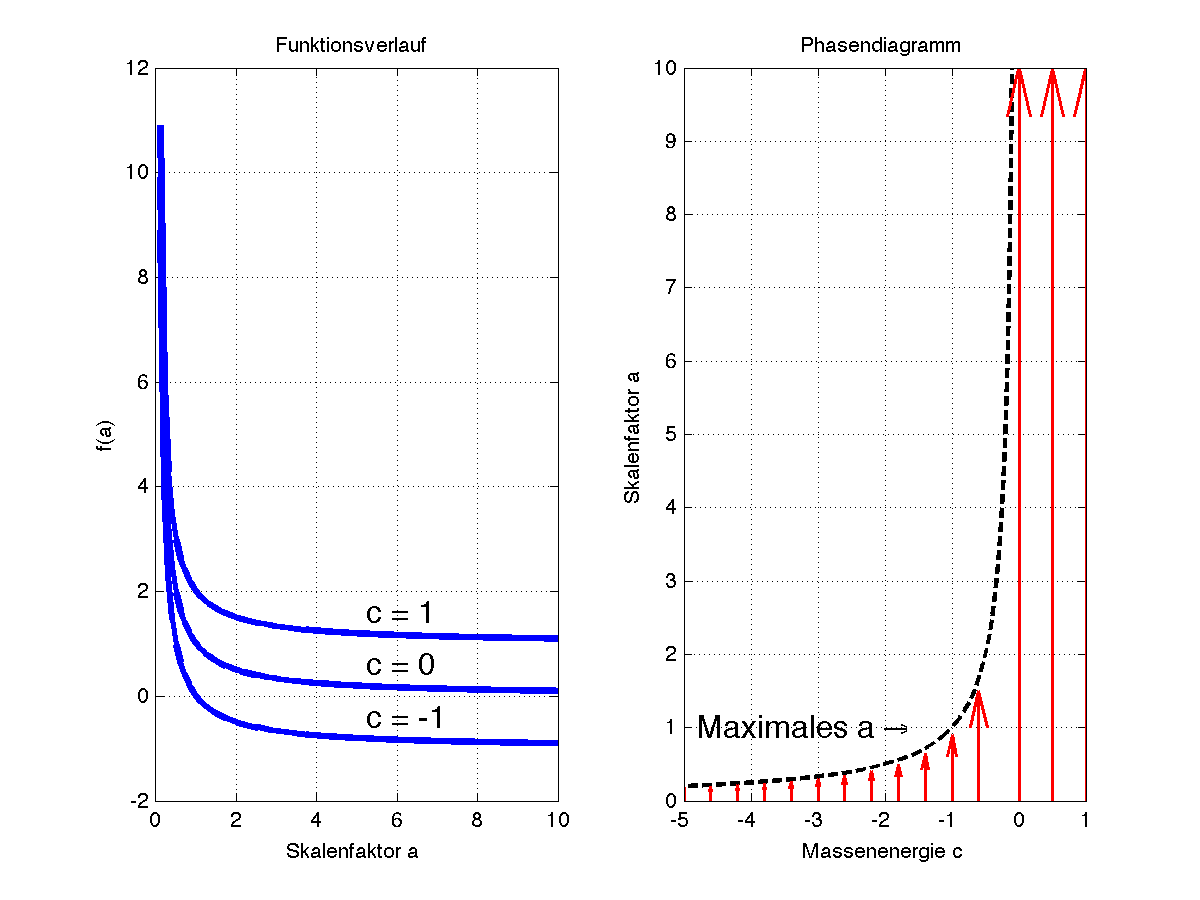
\includegraphics[width  = \textwidth]{friedmann/images/phasendiagramm.png}
	\caption{Phasenportrait in Abhängigkeit der Gesamtenergie c
		\label{friedmann:phasenportrait}}
\end{figure}%

%In \ref{friedmann:friedmannGleichung} sind die Differentialgleichungen in Abhängigkeit von c in MatLab numerisch aufgelöst werden. 
%
%\begin{figure}[h]
%	\centering
%	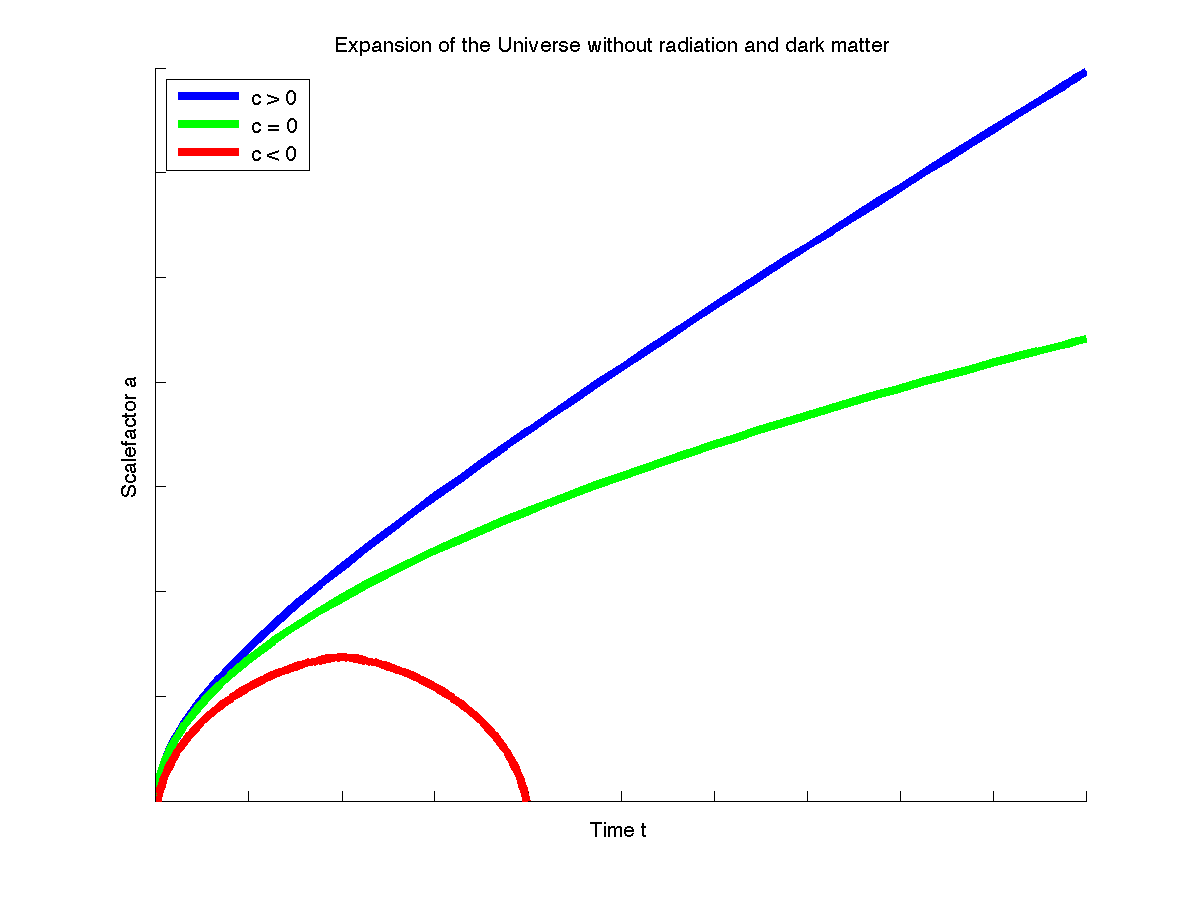
\includegraphics[width =  \textwidth]{friedmann/images/friedmann_ordinary_matter.png}
%	\caption{Verhalten des Universums in Abhängigkeit von der Zeit $t$
%		\label{friedmann:friedmannGleichung}}
%\end{figure}%
	
\section{Relativistischer Ansatz}
Die bisher gemachten Überlegungen berücksichtigen nur die klassische oder newtonsche Physik, tatsächlich spielen die relativistischen Gesetze Einstein's eine wesentliche Rolle bei der Beschreibung des Kosmos.
Im vorhergehenden Abschnitt haben wir die Bedeutung der Massendichte "gewöhnlicher", sogenannter baryonischer Masse kennengelernt. Im relativistischen Ansatz geht es nun darum, die Geometrie des Raumes mit den Energiedichten in einen Zusammenhang zu bringen.
Die bereits hergeleitete Formel können wir so umschreiben, dass die linke Seite etwas mit der Geometrie des Raumes zu tun hat, während die rechte Seite die Energiedichte repräsentiert.
\begin{equation}
\left(\frac{\dot{a}}{a} \right)^2 - \frac{c}{a^2} = \frac{8 \pi G}{3} \rho 
\label{friedmann:Einstein}
\end{equation}

\subsection{Energiedichte}
Wie wir wissen, existiert im Weltall nicht nur sichtbare, sondern auch dunkle Materie und Strahlung. Dunkle Materie verhält sich in Bezug auf die gravitative Wirkung ähnlich wie sichtbare Materie, und deshalb wird im weiteren nicht weiter darauf eingegangen.
Anders verhält es sich mit der kosmischen Strahlung in Bezug auf die Dynamik des Kosmos. Wir schreiben


\[ E_{str} = \frac{h c}{\lambda} \]

wobei $h$ die \textbf{Planksche Konstante}, $c$ die \textbf{Lichtgeschwindigkeit} und $\lambda$ die \textbf{Wellenlänge} des Photons ist.
Nun ist die Energie der Strahlung (z.B. eines Photons) in einem sich ausdehnenden Universum nicht konstant, sondern ändert sich mit der Zeit. 
Denn, vergrössert sich die Raumzeit während der Laufzeit um einen Faktor n, so geschieht dies auch mit der Wellenlänge des Strahls.
Das bedeutet, dass die Energie eines Photons umgekehrt proportional zum Skalenfaktor a ist. Für die Energiedichte der Strahlung bedeutet dies, dass sie sich nicht nur kubisch wie bei der baryonischen Materie ändert, sondern mit vierter Potenz.
\begin{equation}
\rho_{str} = \frac{\nu}{a^4}
\end{equation}
In die Gleichung der Energieerhaltung des Universums setzen wir $\rho_{str}$ ein.
\[
\left(\frac{\dot{a}}{a} \right)^2 = \frac{8 \pi G}{3} \frac{\nu}{a^4} + \frac{c_2}{a^2 R^2}
\]
Vereinfacht
\[
\left(\frac{\dot{a}}{a} \right)^2 = \frac{1}{a^4} + \frac{c}{a^2} \Leftrightarrow \dot{a} = \sqrt{\frac{1}{a^2} + c}
\]

Wiederum ist die Differentialgleichung nicht elementar lösbar. Trotzdem können wir sagen, dass für \textbf{kleine} \textit{a's} der \textbf{erste} Term dominiert, während der \textbf{zweite} Term für \textbf{grosse} \textit{a's} dominiert.

Setzen wir die Gesamtenergie des Universums $c$ gleich null, findet sich die Lösung	\[\left(\frac{\dot{a}}{a} \right)^2 = \frac{1}{a^4}\]
Um die Gleichung zu lösen, ziehen wir die Quadratwurzel und multiplizieren mit $a$.
\[ \dot{a} = \frac{1}{a} \]
\[\frac{da}{dt} =\frac{1}{a} \Leftrightarrow \frac{dt}{da} = a \]
\[ t = \frac{1}{2} a^{2} \Rightarrow a = \sqrt{2} \quad t^{1/2} \]


\subsection{Geometrie des Raumes}
Wie wir zu beginn des Abschnitts erwähnt haben, muss die  linke Seite der Gleichung \ref{friedmann:Einstein} etwas mit der Geometrie des Raumes zu tun haben.
Der erste Term ist die Hubble-Konstante und beschreibt die Ausdehnung des Raumes. Das heisst
$c$ muss die Krümmung des Raumes wiedergeben.
Wir benennen die Konstante um zu
$-\kappa$ und schreiben die Gleichung neu:


\[ \left(\frac{\dot{a}}{a} \right)^2 + \frac{\kappa}{a^2} = \frac{8 \pi G}{3} \rho  \]

\begin{equation}
\left(\frac{\dot{a}}{a} \right)^2  = \frac{8 \pi G}{3} \rho  - \frac{\kappa}{a^2}
\end{equation}
\begin{table}[h]
\centering
\begin{tabular}{|>{$}r<{$}|>{$}r<{$}|>{$}c<{$}|}
\hline
\kappa&Geometrie&Winkelsumme\: \Delta\\
\hline
+1 & \text{Elliptisch} & > 180^\circ\\
0  & \text{Euklidisch} & =180^\circ\\
-1 & \text{Hyperbolisch} & <180^\circ\\
\hline	
\end{tabular}
\caption{Bedeutung von $\kappa$ für die Geometrie des Raumes}
\end{table} \linebreak
Die Krümmung des Raumes kann durch Messen von Winkelsummen im Dreieck bestimmt werden.

\subsection{Redshift}
Es stellt sich die Frage, wie sich die momentane Ausbreitungsgeschwindigkeit feststellen lässt. Dabei nutzt man die Erkenntnis, dass sich die Wellenlänge von Licht, welches sich durch einen ausdehnenden Raum bewegt, mit dehnt und somit ein anderes Farbspektrum erhält. Diese Verschiebung der Wellenlänge ins Rot nennt man in der Kosmologie Rotverschiebung. Daraus kann man nun die Ausdehnung des Raums während der Zeit, die das Licht reist, ausrechnen. Die Ausbreitungsgeschwindigkeit wird mit der Hubble-Konstante angegeben und beträgt heute 
\[ H_0 = H(t_0) \approx (74.3 \pm 2.1) \frac{km}{s}\frac{1}{Mpc}\]
, wobei $t_0$ für das heutige Weltalter steht.	

\end{refsection}
